\chapter{Two dimensions versus three}
\label{ch:c5}
\begin{keybox}
\textbf{Key idea.} Going from 2-D to 3-D is not a small constant factor.
Every level of refinement multiplies the degrees of freedom by $4$ in
2-D but $8$ in 3-D, the stencil thickens from $9$ to $27$ neighbors, the
matrix nonzeros can overflow 32-bit indexing, and the direct-solver fill
explodes --- which is precisely why 3-D forces the device assembly path
and the \texttt{blockch} solver of Chapter~\ref{ch:c4}.
\end{keybox}

This concept measures the 2-D-vs-3-D growth live on small meshes and
connects it to the device-scale ladders from the dev notes. It is the
capstone of the computational track: it explains \emph{why} everything
in Chapter~\ref{ch:c4} (the device assembly path, the \texttt{blockch}
solver, the matrix-free frontier) exists.

\section{Three things grow at once}

Refine a mesh by one level and the number of elements multiplies by
$2^{\dim}$ --- $4$ in 2-D, $8$ in 3-D. That is the obvious growth. Two
less-obvious ones compound it:

\begin{itemize}[nosep]
  \item \textbf{The stencil thickens.} A node couples to its
        $3^{\dim}-1$ neighbors: $8$ in 2-D (a 9-point stencil), $26$ in
        3-D (a 27-point stencil). For the mixed $(c,\mu)$ system that is
        $\sim\CfiveNnzPerDofTwoD$ nonzeros per dof in 2-D and
        $\sim\CfiveNnzPerDofThreeD$ in 3-D (measured below). The matrix
        is not just bigger --- it is \emph{denser per row}.
  \item \textbf{The direct-solver fill explodes.} A larger 3-D bandwidth
        makes the LU factors fill in far worse than in 2-D --- the cuDSS
        memory ceiling of Chapter~\ref{ch:c4}.
\end{itemize}

\begin{keybox}
\textbf{The compounding.} 2-D dofs grow $\times4$/level and carry
$\sim\!18$ nnz/dof; 3-D dofs grow $\times8$/level and carry $\sim\!50$
nnz/dof. Four levels of refinement is $256\times$ the dofs in 2-D but
$4096\times$ in 3-D --- and each 3-D dof is $\sim3\times$ denser. This is
why a code that is instant in 2-D needs a GPU, a device assembler, and a
scalable solver in 3-D.
\end{keybox}

\section{Run it}

\begin{runbox}
\textbf{Run it.}
\begin{lstlisting}
cd computational/05_two_vs_three
python run.py            # live 2-D vs tiny-3-D + cited ladder (~30-40 s)
\end{lstlisting}
The 3-D level-5 step is a real $\CfiveThreeDdofs$-dof Cahn--Hilliard step
on the box (a few seconds). Compare with \file{EXPECTED.md} and
Fig.~\ref{fig:c5dof}--\ref{fig:c5nnz}.
\end{runbox}

Measured: dofs grow $\times\CfiveDofGrowthTwoD$/level in 2-D and
$\times\CfiveDofGrowthThreeD$/level in 3-D (approaching the theoretical
$4$ and $8$; Fig.~\ref{fig:c5dof}). At comparable size ---
$\CfiveTwoDdofs$ dofs in 2-D versus $\CfiveThreeDdofs$ in 3-D --- the 3-D
matrix has $\CfiveNnzRatio\times$ the nonzeros and the step takes
$\CfiveStepRatio\times$ as long.

\begin{figure}[h]\centering
  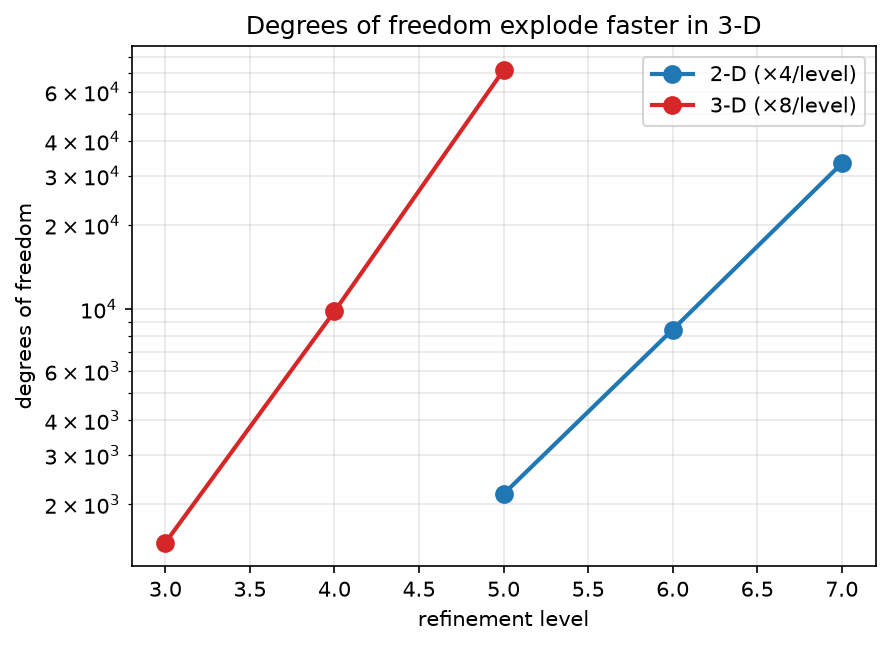
\includegraphics[width=0.62\linewidth]{figures/c5_dofgrowth.png}
  \caption{Degrees of freedom versus refinement level (log scale). Each
    2-D level multiplies dofs by $\sim4$; each 3-D level by $\sim8$. The
    gap widens without bound.}
  \label{fig:c5dof}
\end{figure}

\section{The device-scale ladder}

The live meshes stop at tens of thousands of dofs; production 3-D films
run at \emph{millions}. Figure~\ref{fig:c5nnz} places the cited
device-scale points (dev notes) on the same axes as the live runs, with
the 32-bit index ceiling drawn in.

\begin{itemize}[nosep]
  \item \code{3d\_slab64} ($417{,}792$ dofs, $65$M nnz) is the largest
        cuDSS-stable case on a 48\,GB card --- $3\%$ of the int32 ceiling.
  \item \code{3d\_film128} ($\CfiveFilmDofs$ dofs, $1.02$B nnz) runs on
        \emph{one} 48\,GB card with \texttt{blockch}; cuDSS cannot.
  \item at $(M{=}3,K{=}2)$ production physics, \code{128x128x48}
        ($\CfiveMkOverflowDofs$ dofs) \emph{overflows} the 32-bit nnz
        arithmetic --- which is exactly why the block-masked pattern
        exists (it drops the structural zeros the superset stores).
  \item \code{256x256x128} ($\CfiveNovaDofs$ dofs, $22.8$B nnz) has no
        single-card stored CSR at all --- only matrix-free or multi-GPU.
\end{itemize}

\begin{figure}[h]\centering
  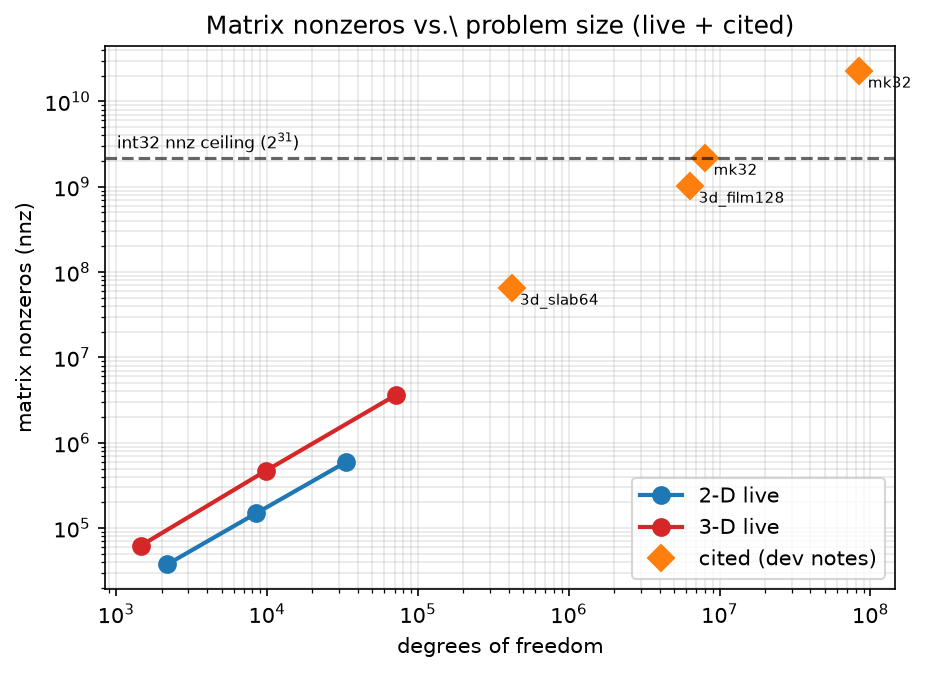
\includegraphics[width=0.72\linewidth]{figures/c5_nnz.png}
  \caption{Matrix nonzeros versus problem size: live 2-D/3-D runs plus
    the cited device-scale points. The dashed line is the 32-bit CSR
    index ceiling ($2^{31}$); the $(M{=}3,K{=}2)$ 128-class films cross
    it, forcing the block-masked pattern, and the Nova-class case
    (22.8\,B nnz) has no stored-CSR form at all.}
  \label{fig:c5nnz}
\end{figure}

\begin{keybox}
\textbf{Measured self-check} (counts are exact; step times are
card-dependent).
\begin{center}\small
\begin{tabular}{lcc}
\toprule
 & 2-D & 3-D \\
\midrule
dofs per level          & $\times\CfiveDofGrowthTwoD$ & $\times\CfiveDofGrowthThreeD$ \\
nnz per dof (stencil)   & $\CfiveNnzPerDofTwoD$ & $\CfiveNnzPerDofThreeD$ \\
\midrule
\multicolumn{3}{l}{\footnotesize at comparable size ($\CfiveTwoDdofs$ vs $\CfiveThreeDdofs$ dofs):} \\
nnz ratio (3-D / 2-D)   & \multicolumn{2}{c}{$\CfiveNnzRatio\times$} \\
step-time ratio         & \multicolumn{2}{c}{$\CfiveStepRatio\times$} \\
\bottomrule
\end{tabular}
\end{center}
\end{keybox}

\section{Code walk-through}

\paragraph{Measuring a real system's size.}
\begin{lstlisting}
dofs, nnz, step_s = _capture_nnz(dim, level)   # one real CH step
row = scaling_row(dim, level)                  # + nnz/dof, mem estimate
\end{lstlisting}
As in Chapter~\ref{ch:c4}, the benchmark assembles the \emph{real}
Cahn--Hilliard Jacobian and reads its nnz --- the true storage the solver
faces, not a formula.

\paragraph{The int32 ceiling.}
\begin{lstlisting}
INT32_MAX = 2**31
int32_headroom(nnz)          # nnz / 2^31: >1 means the CSR overflows
\end{lstlisting}
The CSR index arithmetic is 32-bit; once nnz passes $2^{31}$ the slot
arithmetic overflows, and the code must either mask the pattern down or
go matrix-free.

\section{Explore on your own}

\question{Fit a power law to the live 3-D step times ($\text{step}\sim
\text{dofs}^\alpha$). Is $\alpha$ closer to $1$ (ideal), $1.5$, or worse?
Which stage --- host assembly or the solve --- drives it, and does that
match the C4 story of where 3-D cost lives?}

\question{Compute the crossover level at which a 3-D mesh overtakes a
2-D mesh of the same refinement level in \emph{total nnz}. Then compute
the level at which a uniform 3-D mesh would overflow int32 at
$(M{=}1)$ binary physics --- and compare with the cited $(M{=}3,K{=}2)$
overflow at 128×128×48.}

\question{The block-masked pattern drops structural zeros to fit int32.
Using the cited $(M{=}3,K{=}2)$ mask density ($54/100$ live blocks),
predict the masked nnz for 128×128×48 and check it against the dev
note's $1.16$B. At what mesh does even the \emph{masked} pattern
overflow?}

\question{Estimate the host memory to store the 3-D level-6 CH matrix
($\sim5.7\times10^5$ dofs) from the measured nnz/dof, and compare with
the GPU memory a direct factorization would need (use the C4 fill
behavior). Which runs out first, and on which card?}

\question{An octree mesh (Chapter~\ref{ch:c3}) refined only at the
interfaces changes the 3-D growth law: a surface scales as area, not
volume. Estimate how many dofs an interface-refined 3-D film would have
versus the uniform $\CfiveThreeDdofs$, and argue why adaptivity matters
far more in 3-D than in 2-D.}
